% Copyright (C) 2014-2023 by Thomas Auzinger <thomas@auzinger.name>

% TODO: remove draft
\documentclass[draft,final]{vutinfth} % Remove option 'final' to obtain debug information.

% Load packages to allow in- and output of non-ASCII characters.
\usepackage{lmodern}        % Use an extension of the original Computer Modern font to minimize the use of bitmapped letters.
\usepackage[T1]{fontenc}    % Determines font encoding of the output. Font packages have to be included before this line.
\usepackage[utf8]{inputenc} % Determines encoding of the input. All input files have to use UTF8 encoding.

% Extended LaTeX functionality is enables by including packages with \usepackage{...}.
\usepackage{amsmath}    % Extended typesetting of mathematical expression.
\usepackage{amssymb}    % Provides a multitude of mathematical symbols.
\usepackage{mathtools}  % Further extensions of mathematical typesetting.
\usepackage{microtype}  % Small-scale typographic enhancements.
\usepackage[inline]{enumitem} % User control over the layout of lists (itemize, enumerate, description).
\usepackage{multirow}   % Allows table elements to span several rows.
\usepackage{booktabs}   % Improves the typesetting of tables.
\usepackage{subcaption} % Allows the use of subfigures and enables their referencing.
\usepackage[ruled,linesnumbered,algochapter]{algorithm2e} % Enables the writing of pseudo code.
\usepackage[usenames,dvipsnames,table]{xcolor} % Allows the definition and use of colors. This package has to be included before tikz.
\usepackage{nag}       % Issues warnings when best practices in writing LaTeX documents are violated.
\usepackage{todonotes} % Provides tooltip-like todo notes.
\usepackage{hyperref}  % Enables hyperlinking in the electronic document version. This package has to be included second to last.
\usepackage[acronym,toc]{glossaries} % Enables the generation of glossaries and lists of acronyms. This package has to be included last.

% custom packages
\usepackage{threeparttable}
\usepackage{makecell}
\usepackage{amsthm}
\usepackage{tikz}
\usetikzlibrary{arrows.meta}

\newtheorem{theorem}{Theorem}
\newtheorem{definition}{Definition}

% Define convenience functions to use the author name and the thesis title in the PDF document properties.
\newcommand{\authorname}{Othmar Lechner} % The author name without titles.
\newcommand{\thesistitle}{T-RACE: Tracing race condition attacks between Ethereum transactions.} % The title of the thesis. The English version should be used, if it exists.

% Set PDF document properties
\hypersetup{
    pdfpagelayout   = TwoPageRight,           % How the document is shown in PDF viewers (optional).
    linkbordercolor = {Melon},                % The color of the borders of boxes around hyperlinks (optional).
    pdfauthor       = {\authorname},          % The author's name in the document properties (optional).
    pdftitle        = {\thesistitle},         % The document's title in the document properties (optional).
    pdfsubject      = {Subject},              % The document's subject in the document properties (optional).
    pdfkeywords     = {a, list, of, keywords} % The document's keywords in the document properties (optional).
}

\setpnumwidth{2.5em}        % Avoid overfull hboxes in the table of contents (see memoir manual).
\setsecnumdepth{subsection} % Enumerate subsections.

\nonzeroparskip             % Create space between paragraphs (optional).
\setlength{\parindent}{0pt} % Remove paragraph indentation (optional).

\makeindex      % Use an optional index.
\makeglossaries % Use an optional glossary.
%\glstocfalse   % Remove the glossaries from the table of contents.

% Set persons with 4 arguments:
%  {title before name}{name}{title after name}{gender}
%  where both titles are optional (i.e. can be given as empty brackets {}).
\setauthor{}{\authorname}{}{male}
\setadvisor{Ass.Prof.in Dipl.-Ing.in Mag.a rer.soc.oec. Dr.in techn.}{Monika di Angelo}{}{female}

% For bachelor and master theses:
\setfirstassistant{Ao.Univ.Prof. Dr.}{Gernot Salzer}{}{male}
% \setsecondassistant{Pretitle}{Forename Surname}{Posttitle}{male}
% \setthirdassistant{Pretitle}{Forename Surname}{Posttitle}{male}

% For dissertations:
% \setfirstreviewer{Pretitle}{Forename Surname}{Posttitle}{male}
% \setsecondreviewer{Pretitle}{Forename Surname}{Posttitle}{male}

% For dissertations at the PhD School and optionally for dissertations:
% \setsecondadvisor{Ao.Univ.Prof. Dipl.-Ing. Dr.techn.}{Gernot Salzer}{}{male} % Comment to remove.

% Required data.
\setregnumber{11841833}
\setdate{01}{01}{2001} % Set date with 3 arguments: {day}{month}{year}.
\settitle{\thesistitle}{T-RACE: Eine Analyse von race condition Angriffen bei Ethereum Transaktionen} % Sets English and German version of the title (both can be English or German). If your title contains commas, enclose it with additional curvy brackets (i.e., {{your title}}) or define it as a macro as done with \thesistitle.
% \setsubtitle{Optional Subtitle of the Thesis}{Optionaler Untertitel der Arbeit} % Sets English and German version of the subtitle (both can be English or German).

% Select the thesis type: bachelor / master / doctor.
% Bachelor:
% \setthesis{bachelor}
%
% Master:
\setthesis{master}
% TODO: dipl. or master?
\setmasterdegree{dipl.} % dipl. / rer.nat. / rer.soc.oec. / master
%
% Doctor:
%\setthesis{doctor}
%\setdoctordegree{rer.soc.oec.}% rer.nat. / techn. / rer.soc.oec.

% For bachelor and master:
\setcurriculum{Software Engineering \& Internet Computing}{Software Engineering \& Internet Computing} % Sets the English and German name of the curriculum.

% Optional reviewer data:
\setfirstreviewerdata{Affiliation, Country}
\setsecondreviewerdata{Affiliation, Country}


\begin{document}

\frontmatter % Switches to roman numbering.
% The structure of the thesis has to conform to the guidelines at
%  https://informatics.tuwien.ac.at/study-services

\addtitlepage{naustrian} % German title page.
\addtitlepage{english} % English title page.
\addstatementpage

\begin{danksagung*}
    \todo{Ihr Text hier.}
\end{danksagung*}

\begin{acknowledgements*}
    \todo{Enter your text here.}
\end{acknowledgements*}

\begin{kurzfassung}
    \todo{Ihr Text hier.}
\end{kurzfassung}

\begin{abstract}
    \todo{Enter your text here.}
\end{abstract}

% Select the language of the thesis, e.g., english or naustrian.
\selectlanguage{english}

% Add a table of contents (toc).
\tableofcontents % Starred version, i.e., \tableofcontents*, removes the self-entry.

% Switch to arabic numbering and start the enumeration of chapters in the table of content.
\mainmatter

\chapter{Introduction}
\todo{Enter your text here.}

\iffalse
    \section{Related work}

    Interesting things:
    - name
    - source is available?
    - does it use RPC / instrumentation / native tracing?
    - does it detect some kind of frontrunning

    See table \ref{tab:blockchain_history_analyzers}.


    % TODO: is there related work in the parallel EVM field? TOD is highly relevant for this
    % https://ieeexplore.ieee.org/abstract/document/10102454


    \begin{table}[h]
        \begin{center}
            \begin{tabular}{ | l | c  | c | c | c | }
                \hline
                Tool/Authors                                     & Scope            \\ \hline
                EthScope \cite{wu_time-travel_2022}              & Generalized      \\ \hline
                TokenScope \cite{chen_tokenscope_2019}           & ERC-20 tokens    \\ \hline
                TXSPECTOR \cite{zhang_txspector_2020}            & Generalized      \\ \hline
                Horus \cite{ferreira_torres_eye_2021}            & Generalized      \\ \hline
                SODA \cite{chen_soda_2020}                       & Generalized      \\ \hline
                DEFIER \cite{su_evil_2021}                       & Generalized      \\ \hline
                Zhou et al. \cite{zhou_ever-evolving_2020}       & Generalized      \\ \hline
                Perez et al. \cite{perez_smart_2021}             & Generalized      \\ \hline
                Wang et al. \cite{wang_impact_2022}              & Sandwich attacks \\ \hline
                Erebus-redgiant \cite{zhang_combatting_2023}     & Frontrunning     \\ \hline
                Frontrunner Jones \cite{torres_frontrunner_2021} & Frontrunning     \\ \hline
            \end{tabular}
            \caption{Blockchain history analysis references. Generalized means, that the data collection and analysis framework is not tailored to specific vulnerabilities.}
            \label{tab:blockchain_history_analyzers}
        \end{center}
    \end{table}
    \todo{Better caption}

    \section{Related approaches}

    \subsection{Combatting paper - Erebus-redgiant}

    How do they replay potential attack/victim transactions?

    Their framework allows forking at a specific block and tx index.

    PrepareStateAndContext - replays up to tx index.


    They skip potential victim transactions if:

    \begin{enumerate}
        \item error victim transactions (\todo{Are these failed transactions in Ethereum, or error somewhere in their framework? If it's the first, why???})
        \item "filtered" transactions \todo{What are these?}
        \item unverified contracts in victim transactions
        \item victim tx is contract creation (why???). But a good label :)
        \item victim tx is ether transfer
        \item no overlap with attack tx (compare sets of contracts/accounts)
        \item no dependency (storage and balance dependencies, but seem to ignore dependencies within reverted calls)
    \end{enumerate}

    Replaying in the attack free scenario:

    \begin{enumerate}
        \item take attack tx state (I guess prestate)
        \item take victim context (I guess block environment, timestamp, ...)
        \item apply "prerequesites" - all previous transactions from the same sender within (attack, victim-1)?
        \item apply + trace victim tx
        \item apply + trace attack tx
    \end{enumerate}

    For prerequisites, refer to \href{https://github.com/Troublor/erebus-redgiant/blob/4544163f0c6a369b35c3237851f482d240fa7bbd/dataset/tx_history_test.go#L42-L53}.

    Problems with this approach:

    \begin{enumerate}
        \item Prerequisites is an arbitrary choice
              \subitem what if prerequisites have collisions with the attack?
              \subitem what if prerequisites depend on other transactions that were not replayed?
              \subitem what if victim tx depends on other transactions that were not replayed?
        \item all transactions share the same context
              \subitem attack tx is moved to different context
              \subitem prerequisites are potentially moved to different context
              \subitem (victim tx stays in same context \checkmark)
        \item replay is done with a different environment
    \end{enumerate}
\fi

TBD.

\section{Contributions}


\begin{itemize}
    \item Precise definition of TOD in the context of blockchain transaction analysis.
    \item Theoretical discussion of TOD, including compilation of instructions that can cause TOD.
    \item Methodology to mine potential TOD transaction pairs using only the RPC interface of an archive node, rather than requiring local access to it.
\end{itemize}

\chapter{Background}

This chapter gives background knowledge on Ethereum, that is helpful to follow the remaining paper. We also introduce a notation for these concepts.

\section{Ethereum}

Ethereum is a blockchain, that can be characterized as a "transactional singleton machine with shared-state". \cite[p.1]{wood_ethereum_2024} By using a consensus protocol, a decentralized set of nodes agrees on a globally shared state. This state contains two types of accounts: \emph{externally owned accounts} (EOA) and \emph{contract accounts} (also referred to as smart contracts). The shared state is modified by executing \emph{transactions}. \cite{tikhomirov_ethereum_2018}

\section{World State}

Similar to \cite[p.3]{wood_ethereum_2024}, we will refer to the shared state as \emph{world state}. The world state maps each 20 byte address to an account state, containing a \emph{nonce}, \emph{balance}, \emph{storage} and \emph{code}\footnote{Technically, the account state only contains hashes that identify the storage and code, not the actual storage and code. This distinction is not relevant in this paper, therefore we simply refer to them as nonce and code.}. They store following data \cite[p.4]{wood_ethereum_2024}:

\begin{itemize}
    \item \emph{nonce}: For EOAs, this is the number of transactions submitted by this account. For contract accounts, this is the number of contracts created by this account.
    \item \emph{balance}: The value of Wei this account owns, a smaller unit of Ether.
    \item \emph{storage}: The storage allows contract accounts to persistently store information across transactions. It is a key-value mapping where both, key and value, are 256 bytes long. For EOAs, this is empty.
    \item \emph{code}: For contract accounts, the code is a sequence of EVM instructions.
\end{itemize}

We denote the world state as $\sigma$, the account state of an address $a$ as $\sigma(a)$ and the nonce, balance, storage and code as $\sigma(a)_n$, $\sigma(a)_b$, $\sigma(a)_s$ and $\sigma(a)_c$ respectively. For the value at a storage slot $k$ we write $\sigma(a)_s[k]$. We will also an alternative notation $\sigma(K)$, where we combine the identifiers of a state value to a single key $K$, which simplifies further definitions. We have the following equalities between the two notations:

\begin{align*}
    \sigma(a)_n    & = \sigma(("nonce", a))      \\
    \sigma(a)_b    & = \sigma(("balance", a))    \\
    \sigma(a)_c    & = \sigma(("code", a))       \\
    \sigma(a)_s[k] & = \sigma(("storage", a, k)) \\
\end{align*}

\section{EVM}

The Ethereum Virtual Machine (EVM) is used to execute code in Ethereum. It executes instructions, that can access and modify the world state. The EVM is Turing-complete, except that it is executed with a limited amount of \emph{gas} and each instruction costs some gas. When it runs out of gas, the execution will halt. \cite[p.14]{wood_ethereum_2024} For instance, this prevents execution of infinite loops, as it would use infinitely much gas and thus exceed the gas limit.

Most EVM instructions are formally defined in. \cite[p.30-38]{wood_ethereum_2024} However, the Yellowpaper currently does not include the changes from the Cancun upgrade \cite{noauthor_history_2024}, therefore we will also refer to the informal descriptions available on \href{https://www.evm.codes/}{evm.codes}. \cite{smlxl_evm_2024}

\section{Transactions}

A transaction can modify the world state by transferring Ether and executing EVM code. It must be signed by the owner of an EOA and contains following data relevant to our work:

\begin{itemize}
    \item \emph{sender}: The address of the transaction sender\footnote{The sender is implicitly given through a valid signature and the transaction hash. \cite[p.25-27]{wood_ethereum_2024} We are only interested in transactions that are included in the blockchain, thus the signature must be valid and the transaction's sender can always be derived.}.
    \item \emph{recipient}: The destination address.
    \item \emph{value}: The value of Wei that should be transferred from the sender to the recipient.
    \item \emph{gasLimit}: The maximum number of gas, that can be used for the execution.
\end{itemize}

If the recipient address is empty, the transaction will create a new contract account. These transactions also include an \emph{init} field, that contains the code to initialize the new contract account.

When the recipient address is given and a value is specified, this will be transferred to the recipient. Moreover, if the recipient is a contract account, it also executes the recipient's code. The transaction can specify a \emph{data} field to pass input data to the code execution. \cite[p.4-5]{wood_ethereum_2024}

% TODO: move \cite to pre/post period.

For every transaction the sender must pay a \emph{transaction fee}. This is composed of a \emph{base fee} and a \emph{priority fee}. Every transaction must pay the base fee. The amount of Wei will be reduced from the sender and not given to any other account. For the priority fee, the transaction can specify if, and how much they are willing to pay. This fee will be taken from the sender and given to the block validator, which is explained in the next section. \cite[p.8]{wood_ethereum_2024}

We denote a transaction as $T$, sometimes adding a subscript $T_A$ to differentiate from another transaction $T_B$.

\section{Blocks}

The Ethereum blockchain consists of a sequence of blocks, where each block builds upon the state of the previous block. To achieve consensus about the canonical sequence of blocks in a decentralized network of nodes, Ethereum uses a consensus protocol. In this protocol, validators build and propose blocks to be added to the blockchain. \cite{noauthor_gasper_2023} It is the choice of the validator, which transactions to include in a block, however they are incentivized to include transactions that pay high transaction fees, as they receive the fee. \cite[p.8]{wood_ethereum_2024}

Each block consists of a block header and a sequence of transactions. We denote the nth block of the blockchain as $B_n$ and the sequence of transactions it includes as $T(B_n) = (T_1, T_2, \dots, T_m)$.

\section{Transaction submission}

This section discusses, how a transaction signed by an EOA ends up being included in the blockchain.

Traditionally, the signed transaction is broadcasted to the network of nodes, which temporarily store them in a \emph{mempool}, a collection of pending transactions. The current block validator then picks transactions from the mempool and includes them in the next block. With this submission method, the pending transactions in the mempool are publicly known to the nodes in the network, even before being included in the blockchain. This time window will be important for our discussion on frontrunning, as it gives nodes time to react on a transaction before it becomes part of the blockchain. \cite{eskandari_sok_2020}

A different approach, the Proposer-Builder Separation (PBS) has become more popularity recently: Here, we separate the task of collecting transactions and building blocks with them from the task of proposing them as a validator. A user submits their signed transaction or transaction bundle to a block builder. The block builder has a private mempool and uses it to create profitable blocks. Finally, the validator picks one of the created blocks and adds it to the blockchain. \cite{heimbach_ethereums_2023}

\section{Transaction execution}

In Ethereum, transaction execution is deterministic. \cite[p.9]{wood_ethereum_2024} Transactions can access the world state and their block environment, therefore their execution can depend on these values. After executing a transaction, the world state is updated accordingly.

We denote a transaction execution as $\sigma \xrightarrow{T} \sigma\prime$, implicitly letting the block environment correspond to the transaction's block. Furthermore, we denote the state change by a transaction $T$ as $\Delta_T$, with $prestate(\Delta_T) = \sigma$ being the world state before execution and $poststate(\Delta\sigma_T) = \sigma\prime$ the world state after the execution of $T$.

For two state changes $\Delta_{T_A}$ and $\Delta_{T_B}$, we say that $\Delta_{T_A} = \Delta_{T_B}$ if they changed the same set of state fields and the pre- and poststate for these changed fields is equal, otherwise $\Delta_{T_A} \neq \Delta_{T_B}$. For instance, if both $\Delta_{T_A}$ and $\Delta_{T_B}$ modified only the storage slot $\sigma(a)_s[k]$, and both changed it from the value $x$ to the value $y$, we would call them equal. If $\Delta_{T_B}$ changed it from $x\prime$ to $y$, or from $x$ to $y\prime$ or even modified a different storage slot $\sigma(a)_s[k\prime]$, we would say $\Delta_{T_A} \neq \Delta_{T_B}$.

We define the set of changed state keys as:

$$changed\_keys(\Delta) \coloneqq \{ K | prestate(\Delta)(K) \neq poststate(\Delta)(K) \}$$

We let the equality $\Delta_{T_A} = \Delta_{T_B}$ be true if following holds, else $\Delta_{T_A} \neq \Delta_{T_B}$:

\begin{align*}
    changed\_keys(\Delta_{T_A})       & = changed\_keys(\Delta_{T_B})                           \\
    \forall K \in changed\_keys\colon &
    prestate(\Delta_{T_A})(K) = prestate(\Delta_{T_B})(K)                                       \\
    \text{ and }                      & poststate(\Delta_{T_B})(K) = poststate(\Delta_{T_B})(K)
\end{align*}

We define $\sigma + \Delta_T$ to be equal to the state $\sigma$, except that every state that was changed by the execution of $T$ is overwritten with the value in $poststate(\Delta_T)$. Similarly, $\sigma - \Delta_T$ is equal to the state $\sigma$, except that every state that was changed by the execution of $T$ is overwritten with the value in $prestate(\Delta_T)$. Formally, these definitions are as follows:

\begin{align*}
    (\sigma + \Delta_T)(K) & \coloneqq
    \begin{cases}
        poststate(\Delta_T)(K), & K \in changed\_keys(\Delta_T) \\
        \sigma(K),              & \text{otherwise}
    \end{cases} \\
    (\sigma - \Delta_T)(K) & \coloneqq
    \begin{cases}
        prestate(\Delta_T)(K), & K \in changed\_keys(\Delta_T) \\
        \sigma(K),             & \text{otherwise}
    \end{cases}
\end{align*}

For instance, if transaction $T$ changed the storage slot 1234 at address 0xabcd from 0 to 100, then $(\sigma + \Delta_T)(\text{0xabcd})_s[1234] = 100$ and $(\sigma - \Delta_T)(\text{0xabcd})_s[1234] = 0$. For all other storage slots we have $(\sigma + \Delta_T)(a)_s[k] = \sigma(a)_s[k] = (\sigma - \Delta_T)(a)_s[k]$.

\section{Nodes}

A node consists of an \emph{execution client} and a \emph{consensus client}. The execution client keeps track of the world state and the mempool and executes transactions. The consensus client takes part in the consensus protocol. For this work, we will use an \emph{archive node}, which is a node that allows to reproduce the state and transactions at any block. \cite{noauthor_nodes_2024}

\section{RPC}

Execution clients implement the Ethereum JSON-RPC specification. \cite{noauthor_ethereum_2024} This API gives remote access to an execution client, for instance to inspect the current block number with \verb|eth_blockNumber| or to execute a transaction without committing the state via \verb|eth_call|. In addition to the standardized RPC methods, we will also make use of methods in the debug namespace, such as \verb|debug_traceBlockByNumber|. While this namespace is not standardized, several execution clients implement these additional methods \cite{noauthor_go-ethereum_2024}\cite{noauthor_rpc_2024}\cite{noauthor_reth_2024}.

\chapter{Transaction order dependency}

In this chapter we discuss our definition of transaction order dependency (TOD) and various properties that come with it. We first lay out the idea of TOD with a basic definition and then show several shortcomings of this simple definition. Based on these insights, we construct a more precise definition that we will use for our analysis.

\section{Approaching TOD}

Intuitively, a pair of transactions $(T_A, T_B)$ is transaction order dependent (TOD), if the original execution order leads to a different result than a reordered execution order. In formal terms, we write this as following:

$$\sigma \xrightarrow{T_A} \sigma_1 \xrightarrow{T_B} \sigma \prime$$
$$\sigma \xrightarrow{T_B} \sigma_2 \xrightarrow{T_A} \sigma \prime \prime$$
$$\sigma \prime \neq \sigma \prime \prime$$

So, starting from an initial state, when we execute first $T_A$ and then $T_B$ it will result in a different state, than when executing $T_B$ and afterwards $T_A$.

We will refer to the execution order $T_A \rightarrow T_B$, the one that occurred on the blockchain, as the \emph{normal} execution order, and $T_B \rightarrow T_A$ as the \emph{reversed} execution order.

\section{Motivating examples}

\todo{Add a motivating example for write-read TOD (e.g. TOD-recipient) and for write-write TOD (e.g. ERC-20 approval).}

\section{Relation to previous works}

In \cite{torres_frontrunner_2021} the authors do not provide a formal definition of TOD. However, for displacement attacks, they include the following check to detect if two transactions fall into this category:

\begin{quote}
    [...] we run in a simulated environment first $T_A$ before $T_V$ and then $T_V$ before $T_A$. We report a finding if the number of executed EVM instructions is different across both runs for $T_A$ and $T_V$, as this means that $T_A$ and $T_V$ influence each other.
\end{quote}

Similar to our intuitive TOD definition, they execute $T_A$ and $T_V$ in different orders and check if it affects the result. In their case, they only check the number of executed instruction, instead of the resulting state. This would miss attacks where the same instructions were executed, but the operands for these instructions in the second transaction changed because of the first transaction.

In \cite{zhang_combatting_2023}, they define an attack as a triple $A = \langle T_a, T_v, T_a^p\rangle$, where $T_a$ and $T_v$ are similar to the $T_A$ and $T_B$ from our definition, and $T_a^p$ is an optional third transaction. They consider the execution orders $T_a \rightarrow T_v \rightarrow T_a^p$ and $T_v \rightarrow T_a \rightarrow T_a^p$. They monitor the transactions to check if the execution order impacts financial gains, which we will discuss later in more detail\todo{Reference section}.

We note that if these two execution orders result in different states, this is not because of the last transaction $T_a^p$, but because of a TOD between $T_a$ and $T_v$. As we always execute $T_a^p$, and transaction execution is deterministic, it only gives a different result if the execution of $T_a$ and $T_v$ gave a different result. Therefore, if the execution order results in different financial gains, then $T_a$ and $T_v$ must be TOD.

\section{Imprecise definitions}

Our intuitive definition of TOD, and the related definitions shown above, are not precise on the semantics of a reordering of transactions and their executions. These make it impossible to apply exactly the same methodology without analyzing the source code related to the papers. We detect three issues, where the definition is not precise enough and show how these were differently interpreted by the two papers.

For the analysis of the tools by \cite{zhang_combatting_2023} and \cite{torres_frontrunner_2021}, we will use the current version of the source codes, \cite{zhang_erebus-redgiant_2023} and \cite{torres_frontrunner_2022} respectively.

\subsection{Intermediary transactions}

To analyze the TOD $(T_A, T_B)$, we are interested in how $T_A$ affected $T_B$. Our intuitive definition did not specify how to handle transactions that occurred between $T_A$ and $T_B$, which we will name \emph{intermediary transactions}.

For instance, let us assume that there was one transaction $T_X$ in between $T_A$ and $T_B$: $\sigma \xrightarrow{T_A} \sigma_A \xrightarrow{T_X} \sigma_{AX} \xrightarrow{T_B} \sigma_{AXB}$. The execution of $T_B$ clearly could depend on both, $T_A$ and $T_X$. When we are interested in the impact of $T_A$ on $T_B$, we need to define what happens with $T_X$.

For executing the normal order, we would have two possibilities:

\begin{enumerate}
    \item $\sigma \xrightarrow{T_A} \sigma_A \xrightarrow{T_X} \sigma_{AX} \xrightarrow{T_B} \sigma_{AXB}$, the same execution as on the blockchain, including the effects of $T_X$.
    \item $\sigma \xrightarrow{T_A} \sigma_A \xrightarrow{T_B} \sigma_{AB}$, leaving out $T_X$ and thus having a normal execution that potentially diverges from the results on the blockchain (as $\sigma_{AB}$ may differ to $\sigma_{AXB}$).
\end{enumerate}

When executing the reverse order, we could make following choices:

\begin{enumerate}
    \item $\sigma \xrightarrow{T_B} \sigma_B \xrightarrow{T_A} \sigma_{BA}$, which ignores $T_X$ and thus may impact the execution of $T_B$.
    \item $\sigma \xrightarrow{T_X} \sigma_X \xrightarrow{T_B} \sigma_{XB} \xrightarrow{T_A} \sigma_{XBA}$, which executes $T_X$ on $\sigma$ rather than $\sigma_A$ and now also includes the effects of $T_X$ for executing $T_A$.
\end{enumerate}

All of these scenarios are possible, but none of them provides a clean solution to solely analyze the impact of $T_A$ on $T_B$, as we always could have some indirect impact from the (non-)execution of $T_X$.

In \cite{zhang_combatting_2023}, this impact of the intermediary transactions is acknowledged and caused a few false positives:

\begin{quote}
    In blockchain history, there could be many other transactions between $T_a$, $T_v$, and $T_p^a$. When we change the transaction orders to mimic attack-free scenarios, the relative orders between $T_a$ (or $T_v$) and other transactions are also changed. Financial profits of the attack or victim could be affected by such relative orders. As a result, the financial profits in the attack-free scenario could be incorrectly calculated, and false-positively reported attacks may be induced, but our manual check shows that such cases are rare.
\end{quote}

Nonetheless, it is not clear, which of the above scenarios they applied for their analysis. The other work, \cite{torres_frontrunner_2021}, does not mention this issue at all.

\todo{Should I move the technical aspects to an appendix?}

\subsubsection{Code analysis of \cite{zhang_combatting_2023}}


As shown in their algorithm 1, they take as input all the executed transactions. They use these transactions and their results in the \verb|searchVictimGivenAttack| method, where \verb|ar| represents the attack transaction and result and \verb|vr| represents the victim transaction and result.

For the normal execution order ($T_a \rightarrow T_v$), they simply use \verb|ar| and \verb|vr| and pass them to their \verb|CheckOracle| method which then compares the resulting states. As \verb|ar| and \verb|vr| are obtained by executing all transactions, they also include the intermediary transactions for these results (similar to our $\sigma \xrightarrow{T_A} \sigma_A \xrightarrow{T_X} \sigma_{AX} \xrightarrow{T_B} \sigma_{AXB}$ case).

For the reverse order ($T_v \rightarrow T_a$), they take the state before $T_a$, i.e. $\sigma$. Then they execute all transactions obtained from the \verb|SlicePrerequisites| method. And finally they execute $T_v$ and $T_a$.

The \verb|SlicePrerequisites| method uses the \verb|hbGraph| built in \verb|StartSession|, which seems to be a graph where each transaction points to the previous transaction from the same EOA. From this graph, it takes all transactions between $T_a$ and $T_v$, that are from the same sender as $T_v$. This interpretation matches the test case "should slide prerequisites correctly" from the source code. As the paper does not mention these prerequisite transactions, we do not know why this subset of intermediary transactions was chosen.

We can conclude, that \cite{zhang_combatting_2023} executes all intermediary transactions for the normal order. However, for the reverse order, they only execute intermediary transactions that are also sent by the victim, but do not execute any other intermediary transactions.

\subsubsection{Code analysis of \cite{torres_frontrunner_2021}}

In the file \verb|displacement.py|, they replay the normal execution order at the lines 154-155, and the reverse execution order at the lines 158-159. They only execute $T_A$ and $T_V$ (in normal and reverse order), but do not execute any intermediate transactions.

\subsection{Block environments}

When we analyze a pair of transactoins $(T_A, T_B)$, it can be, that these are not part of the same block. The execution of these transactoins can depend on the block environment they are executed in, for instance if they access the current block number. Thus, executing $T_A$ or $T_B$ in a different block environment than on the blockchain may alter their behaviour. From our intuitive TOD definition, it is not clear which block environment(s) we use when replaying the transactions in normal and reverse order.

\subsubsection{Code analysis of \cite{zhang_combatting_2023}}

The block environment used to execute all transactions is contained in \verb|ar.VmContext| and as such corresponds to the block environment of $T_a$. This means $T_a$ is executed in the same block environment as on the blockchain, while $T_v$ and the intermediary transactions may be executed in a different block environment.

\subsubsection{Code analysis of \cite{torres_frontrunner_2021}}

In the file \verb|displacement.py| line 151, we see that the emulator uses the same block environment for both transactions. Therefore, at least one of them will be executed in a different block environment than on the blockchain.

\subsection{Initial state $\sigma$}

While our preliminary TOD definition specifies that we start with the same $\sigma$ in both execution orders, it is up to interpretation which world state $\sigma$ is.

\subsubsection{Code analysis of \cite{zhang_combatting_2023}}

The initial state used to execute the first transaction is \verb|ar.State|, which corresponds to the state directly before executing $T_a$. This includes all previous transactions of the same block.

\subsubsection{Code analysis of \cite{torres_frontrunner_2021}}

The emulator is initialized with the block \verb|front_runner["blockNumber"]-1| and no single transactions are executed prior to running the analysis. Therefore, the state cannot include transactions that were executed in the same block before $T_A$.

Similar to the case with the block environment, this could lead to differences between the emulation and the results from the blockchain, when $T_A$ or $T_V$ are impacted by a previous transaction in the same block.

\section{TOD definition}

To address the issues above, we will provide a more precise definition for TOD.

\begin{definition}[TOD]
    Consider a sequence of transactions, with $\sigma$ being the world state right before $T_A$ was executed on the blockchain:

    $$\sigma \xrightarrow{T_A} \sigma_A \xrightarrow{T_{X_1}} \dots \xrightarrow{T_{X_n}} \sigma_{X_n} \xrightarrow{T_B} \sigma_B$$

    Let $\Delta_{T_A}$ and $\Delta_{T_B}$ be the corresponding state changes from executing $T_A$ and $T_B$, and let all transactions be executed in the same block environment as they were executed on the blockchain.

    We say, that $(T_A, T_B)$ is TOD if and only if executing $(\sigma_{X_n} - \Delta_{T_A}) \xrightarrow{T_B} \sigma_B\prime$ produces a state change $\Delta_{T_B\prime}$ with $\Delta_{T_B} \neq \Delta_{T_B\prime}$.
\end{definition}

Intuitively, we take the world state exactly before $T_B$ was executed, namely $\sigma_{X_n}$. We then record the state changes $\Delta_{T_B}$ from executing $T_B$ directly on $\sigma_{X_n}$, the same way it was executed on the blockchain. Then we simulate what would have happened if $T_A$ was not executed before $T_B$ by removing its state changes and executing $T_B$ on $\sigma_{X_n} - \Delta_{T_A}$. If we observe different state changes for $T_B$ when executed with and without the changes of $T_A$, then we know that $T_A$ has an impact on $T_B$ and conclude TOD between $T_A$ and $T_B$. If there are no differences between $\Delta_{T_B}$ and $\Delta_{T_B\prime}$, then $T_B$ behaves the same regardless of $T_A$ and there is no TOD.

We chose to compare the two executions on the state changes $\Delta_{T_B} \neq \Delta_{T_B\prime}$, rather than on the resulting states $\sigma_B \neq \sigma_B\prime$, to detect a wider range of TODs. Comparing on $\sigma_B \neq \sigma_B\prime$ would be sufficient to detect \emph{write-read} TODs, where the first transaction writes some state and the second transaction accesses this state and outputs a different result because of this. However, we are also interested into \emph{write-write} TODs, where $T_A$ writes some state and $T_B$ overwrites the same state with a different value, thus hiding the change by $T_A$.

For example, let $T_A$ write the value $aaaa$ to some storage, s.t. we have $\sigma_{X_n}(a)_s[k] = aaaa$, and $T_B$ write $bbbb$ to the same storage, s.t. we have $\sigma_B(a)_s[k] = bbbb$. When executing $T_B$ last, the world state would have $bbbb$ at this storage slot, and when executing $T_A$ last, it would be $aaaa$. Therefore, the resulting world state is dependent on the order of $T_A$ and $T_B$. To check for this case, we compare the prestates of each change in $\Delta_{T_B}$ and $\Delta_{T_B\prime}$. In our example, when executing $T_B$ on $\sigma_{X_n}$ we would have $prestate(\Delta_{T_B})(a)_s[k] = aaaa$ (as the changes from $T_A$ are included in this scenario), but when executing on $\sigma_{X_n} - \Delta_{T_A}$ we have $prestate(\Delta_{T_B\prime})(a)_s[k] = 0000$ (as the changes from $T_A$ are undone in this scenario). Therefore, checking for inequality between the prestates from the state changes $\Delta_{T_B}$ and $\Delta_{T_B\prime}$ can detect write-write TODs.

Our definition does not include \emph{read-write} TODs, i.e. we do not check whether executing $T_B$ before $T_A$ would have an impact on $T_A$. We focus on detecting TOD attacks, in which the attacker tries to insert a transaction prior to some transaction $T$ and impact the behaviour of $T$ with this. Therefore, we assume that the first transaction tries to impact the second transaction, and not ignore the other way round.

\subsection{Definition strengths}

\subsubsection{Performance}

To check if two transactions $T_A$ and $T_B$ are TOD, we need the initial world state $\sigma$ and the state changes from $T_A$, $T_B$ and the intermediary transactions $T_{X_n}$. With the state changes we can compute $\sigma_{X_n} - \Delta_{T_A} = \sigma + \Delta_{T_A} + (\sum_{i=0}^{i=n} \Delta_{T_{X_i}}) - \Delta_{T_A}$ and then execute $T_B$ on this state. Using state changes allows us to check if $T_A$ and $T_B$ are TOD with only one transaction execution, despite including the effects of arbitrary many intermediary transactions.

If we want to check n transactions for TOD, we could execute all n transactions to obtain their state changes. There are $\frac{n^2 - n}{2}$ transaction pairs, thus if we wanted to test each pair for TOD we would end up with a total of $n + \frac{n^2 - n}{2} = \frac{n^2 + n}{2}$ transaction executions. Similar to \cite{torres_frontrunner_2021} and \cite{zhang_combatting_2023}, we can filter irrelevant transactions pairs to drastically reduce the search space.

\subsubsection{Similarity to blockchain executions}

With our definition, the state change $\Delta_{T_B}$ from the normal execution is equivalent to the state change that happend on the blockchain. Also, the reversed order is closely related to the state from the blockchain, as we start with $\sigma_{X_n}$ and only modify the relevant parts for our analysis. Furthermore, we prevent effects from block environment changes by using the same one as on the blockchain.

This contrasts other implementations, where transactions are executed in different block environments than originally, are executed based on a different starting state or ignore the impact of intermediary transactions. All three cases can alter the execution of $T_A$ and $T_B$, such that the result is not closely related to the blockchain anymore.

\subsection{Definition weaknesses}
\label{sec:weaknesses}

An intuitive interpretation of our definition would be, that we compare $T_A \rightarrow T_{X_i} \rightarrow T_B$ with $T_{X_i} \rightarrow T_B$, i.e. reckon what would have happened if $T_A$ was not executed. However, the definition we provide does not perfectly match this concept. Our definition does not consider interactions between $T_A$ and the intermediary transactions $T_{X_i}$.

In the intuitive model, removal of $T_A$ could also impact the intermediary transactions and thus indirectly change the behaviour of $T_B$. Then we would not know if $T_A$ directly impacted $T_B$, or only through some interplay with intermediary transactions. Therefore, excluding the interactions between $T_A$ and $T_{X_i}$ may be desirable, however it can lead to unexpected results if one is not aware of this.

\subsubsection{Undoing state changes of intermediary transactions}

When we analyze a TOD for $(T_A, T_B)$, applying $\sigma_{X_n} - \Delta_{T_A}$ could undo state changes done by the intermediary transactions, if $T_A$ modifies the same state keys as some intermediary transaction $T_X$.

For instance, consider the three transactions $T_A$, $T_X$ and $T_B$:

\begin{enumerate}
    \item $T_A$: sender $a$ transfers 5 Ether to address $b$.
    \item $T_X$: sender $x$ transfers 5 Ether to address $b$.
    \item $T_B$: sender $b$ transfers 5 Ether to address $y$.
\end{enumerate}

If we start with a state $\sigma$ where both $a$ and $x$ have 5 Ether and all other accounts have 0, then executing all three transactions would result in the state $\sigma(y)_b = 5 eth$. If we think about the case where $T_A$ would not be executed, i.e. the reverse order, we would get the same result.

However, when we compute $(\sigma_{X_n} - \Delta_{T_A})$ we would overwrite the balance of $b$ in $\sigma_{X_n}$ and set it to 0. Undoing the changes of $T_A$ inadvertently also undoes the changes by $T_X$. If we execute $T_B$ on the resulting state, it would fail.

\subsubsection{Indirect dependencies}

Similar to the previous example, we can also get an unrealistic state when there is a TOD between $T_A$ and some intermediary transaction $T_X$.

Consider the same scenario as before, except that now $T_A$ sends the 5 Ether to $x$ and $x$ initially also has 0 Ether.

In the normal scenario, $a$ would send $x$ 5 Ether ($T_A$), $x$ would forward 5 Ether to $b$ ($T_X$) and finally $b$ would forward these to $y$. If $T_A$ would not exist, then $T_X$ and $T_B$ would both fail because of insufficient funds.

However, when we compute $(\sigma_{X_n} - \Delta_{T_A})$ we would \emph{not} overwrite the balance of $b$ in $\sigma_{X_n}$, as $T_A$ did not modify this balance. Thus, $T_B$ would succeed.

\begin{enumerate}
    \item $T_A$: sender $a$ transfers 5 Ether to address $b$.
    \item $T_X$: sender $x$ transfers 5 Ether to address $b$.
    \item $T_B$: sender $b$ transfers 5 Ether to address $y$.
\end{enumerate}

When we analyze a TOD for $(T_A, T_B)$, applying $\sigma_{X_n} - \Delta_{T_A}$ could lead to an unrealistic state if $T_A$ modifies the same state keys as some intermediary transaction $T_X$.

\section{State collisions}

We denote state accesses by a transaction $T$ as a set of state keys $R_T = \{ K_1, \dots, K_n \}$ and state modifications as $W_T = \{ K_1, \dots, K_m \}$.

We define the state collisions of two transactions as:

$$collisions(T_A, T_B) = (W_{T_A} \cap R_{T_B}) \cup (W_{T_A} \cap W_{T_B})$$

With $W_{T_A} \cap R_{T_B}$ we include write-read collisions, where $T_A$ modifies some state and $T_B$ accesses the same state. With $W_{T_A} \cap W_{T_B}$ we include write-write collisions, where both transactions write to the same state location, for instance to the same storage slot. We do not include $R_{T_A} \cap W_{T_B}$, as we also did not include read-write TOD in our TOD defintion.

\section{TOD candidates}

We will refer to a transaction pair $(T_A, T_B)$, where $T_A$ was executed before $T_B$ and $collisions(T_A, T_B) \neq \emptyset$ as a TOD candidate.

A TOD candidate is not necessarily TOD, for instance consider the case that $T_B$ only reads the value that $T_A$ wrote but never uses it for any computation. This would be a TOD candidate, as they have a collision, however the result of executing $T_B$ is not impacted by this collision.

Conversely, if $(T_A, T_B)$ is TOD, then $(T_A, T_B)$ must also a TOD candidate. For a write-write TOD, this is the case, because both $T_A$ and $T_B$ write to the same state, therefore we have $W_{T_A} \cap W_{T_B} \neq \emptyset$. If we have a write-read TOD, then $T_B$ reads some state that $T_A$ wrote, hence $W_{T_A} \cap R_{T_B} \neq \emptyset$.

Therefore, the set of all TOD transaction pairs is a subset of all TOD candidates.

\section{Causes of state collisions}

This section discusses, what can cause two transactions $T_A$ and $T_B$ to have state collisions. To do so, we show the ways a transaction can access and modify the world state.

\subsection{Causes with code execution}

When the recipient of a transaction is a contract account, it will execute the recipient's code. The code execution can access and modify the state through several instructions. By inspecting the EVM instruction definitions \cite[p.30-38]{wood_ethereum_2024}\cite{smlxl_evm_2024}, we compiled a list of instructions that can access and modify the world state.

In table \ref{tab:state_reading_instructions} we see the instructions, that can access the world state. For most, the reason of the access is clear, for instance \verb|BALANCE| needs to access the balance of the target address. Less obvious is the nonce access of several instructions, which is because the EVM uses the nonce (among other things) to check if an account already exists\cite[p.4]{wood_ethereum_2024}. For CALL, CALLCODE and SELFDESTRUCT, this is used to calculate the gas costs. \cite[p.37-38]{wood_ethereum_2024} For CREATE and CREATE2, this is used to prevent creating an account at an already active address \cite[p.11]{wood_ethereum_2024}\footnote{In the Yellowpaper, the check for the existence of the recipient for CALL, CALLCODE and SELFDESTRUCT is done via the \emph{DEAD} function. For CREATE and CREATE2, this is done in the F condition at equation (113).}.

In table \ref{tab:state_writing_instructions} we see instructions that can modify the world state.

\begin{table}[h]
    \begin{center}
        \begin{tabular}{ | l | c  | c | c | c | }
            \hline
            Instruction  & Storage    & Balance    & Code       & Nonce      \\ \hline
            SLOAD        & \checkmark &            &            &            \\ \hline
            BALANCE      &            & \checkmark &            &            \\ \hline
            SELFBALANCE  &            & \checkmark &            &            \\ \hline
            CODESIZE     &            &            & \checkmark &            \\ \hline
            CODECOPY     &            &            & \checkmark &            \\ \hline
            EXTCODECOPY  &            &            & \checkmark &            \\ \hline
            EXTCODESIZE  &            &            & \checkmark &            \\ \hline
            EXTCODEHASH  &            &            & \checkmark &            \\ \hline
            CALL         &            & \checkmark & \checkmark & \checkmark \\ \hline
            CALLCODE     &            & \checkmark & \checkmark & \checkmark \\ \hline
            STATICCALL   &            &            & \checkmark &            \\ \hline
            DELEGATECALL &            &            & \checkmark &            \\ \hline
            CREATE       &            & \checkmark & \checkmark & \checkmark \\ \hline
            CREATE2      &            & \checkmark & \checkmark & \checkmark \\ \hline
            SELFDESTRUCT &            & \checkmark & \checkmark & \checkmark \\ \hline
        \end{tabular}
        \caption[State accessing instructions]{Instructions that access state. A checkmark indicates, that the execution of this instruction can depend on this state type.}
        \label{tab:state_reading_instructions}
    \end{center}
\end{table}

\begin{table}[h]
    \begin{center}
        \begin{tabular}{ | l | c  | c | c | c | }
            \hline
            Instruction  & Storage    & Balance    & Code       & Nonce      \\ \hline
            SSTORE       & \checkmark &            &            &            \\ \hline
            CALL         &            & \checkmark &            &            \\ \hline
            CALLCODE     &            & \checkmark &            &            \\ \hline
            CREATE       &            & \checkmark & \checkmark & \checkmark \\ \hline
            CREATE2      &            & \checkmark & \checkmark & \checkmark \\ \hline
            SELFDESTRUCT & \checkmark & \checkmark & \checkmark & \checkmark \\ \hline
        \end{tabular}
        \caption[State modifying instructions]{Instructions that modify state. A checkmark indicates, that the execution of this instruction can modify this state type.}
        \label{tab:state_writing_instructions}
    \end{center}
\end{table}

\subsection{Causes without code execution}

Some state accesses and modifications are inherent to transaction execution. To pay for the transaction fees, the balance of the sender is accessed and modified. When a transaction transfers some Wei from the sender to the recipient, it als modifies the recipient's balance. To check if the recipient is a contract account, the transaction also needs to access the code of the recipient. And finally, it also verfies the sender's nonce and increments it by one. \cite[p.9]{wood_ethereum_2024}

\subsection{Relevant collisions for attacks}
\label{sec:relevant-collisions}

The previous sections list possible ways to access and modify the world state. Previous studies have focused on storage and balance collisions, however they did not discuss if or why code and nonce collisions are not important\todo{Reference some of them}. Here, we try to argue, why only storage and balance collisions are relevant for TOD attacks and code and nonce collisions can be neglected.

The idea of an TOD attack is, that an attacker impacts the execution of some transaction $T_B$, by placing a transaction $T_A$ before it. To have some impact, there must be a write-write or write-read collisions between $T_A$ and $T_B$. Therefore, our scenario is that we start from some (vicim) transaction $T_B$ and try to create impactful collisions with a new transaction $T_B$. We assume some set $A$ to be the set of codes and nonces that $T_B$ accesses and writes.

Let us first focus on the instructions, that could modify the accessed codes and nonces in $A$, namely \verb|SELFDESTRUCT|, \verb|CREATE| and \verb|CREATE2|. Since the EIP-6780 update\cite{ballet_eip-6780_2023}, \verb|SELFDESTRUCT| only destroys a contract if the contract was created in the same transaction. Therefore, \verb|SELFDESTRUCT| can only modify a code and nonce within the same transaction, but cannot be used to attack an already submitted transaction $T_B$. The instructions to create a new contract, \verb|CREATE| and \verb|CREATE2|, both use the sender's address for the calculation of the new contract account's address, and both fail when there is already a contract at the target address. \cite[p.11]{wood_ethereum_2024} Therefore, we can only modify the code if the contract did not exist previously. If this is the case, it is unlikely that $T_B$ would make a transaction to exactly this attacker-related address. Therefore, none of these instructions is usable for a TOD attack via code or nonce collisions. A similar argument can be made about contract creation directly via the transaction and some init code.

Apart from instructions, the nonces of an EOA can also be increased by transactions themselves. The only way that $T_B$ can access the nonce of an EOA is through the gas cost calculation when sending Ether to this address. The calculation returns a different cost if the recipient already exists, or has to be newly created. Thus, an attack would be that $T_B$ transfers some Ether to an attacker controlled EOA address $a$ which does not yet exist, and the attacker creates the account at addres $a$ in $T_A$, which slightly increases the gas cost for $T_B$. Again, this attack seems negligible.

Therefore, the remaining attack vectors are \verb|SSTORE|, to modify the storage of an account, and \verb|CALL|, \verb|CALLCODE|, \verb|SELFDESTRUCT| and Ether transfer transactions, to modify the balance of an account.

\section{Everything is TOD}

Our definition of TOD is very broad and marks many transaction pairs as TOD. For instance, if a transaction $T_B$ uses some storage value for a calculation, then the execution likely depends on the transaction that previously has set this storage value. Similarly, when someone wants to transfer Ether, they can only do so when they first received that Ether. Thus, they are dependent on some transaction that gave them this Ether previously.\todo{How do block rewards play into this?}

\begin{theorem}
    For every transaction $T_B$ after the London upgrade\footnote{We reference the London upgrade here, as this introduced the base fee for transactions.}, there exists a transaction $T_A$ such that $(T_A, T_B)$ is TOD.
\end{theorem}

\begin{proof}
    Consider an arbitrary transaction $T_B$ with the sender being some address $sender$. The sender must pay some upfront cost $v_0 > 0$, because they must pay a base fee. \cite[p.8-9]{wood_ethereum_2024}. Therefore, we must have $\sigma(sender)_b \ge v_0$. This requires, that a previous transaction $T_A$ increased the balance of $sender$ to be high enough to pay the upfront cost, i.e. $prestate(\Delta_{T_A})(sender)_b < v_0$ and $poststate(\Delta_{T_A})(sender)_b \ge v_0$.

    When we calculate $\sigma - \Delta_{T_A}$ for our TOD definition, we would set the balance of $sender$ to $prestate(\Delta_{T_A})(sender)_b < v_0$ and then execute $T_B$ based on this state. In this case, $T_B$ would be invalid, as the $sender$ would not have enough Ether to cover the upfront cost.
\end{proof}

Given this property, it is clear that TOD alone is not a useful attack indicator, else we would say that every transaction has been attacked. In the following, we provide some more restrictive definitions.\todo{Frontrunning definitions TBD.}

\iffalse
    \chapter{Frontrunning definitions}

    \todo{Is it important to differentiate between sandwich attacks and displacement attacks?}
    \todo{Should we go from first source to last sink? e.g. in a swap call, we will have multiple LOG events at different levels.}


    For $T_A \rightarrow T_B$:

    \todo{I think this is similar to the $attack altered data$ / taint source from the combatting paper}

    \begin{enumerate}
        \item TOD write point: point, where $T_A$ modifies some state, that is read by $T_B$
        \item TOD read point: point, where $T_B$ reads some state, that was modified by $T_A$
        \item TOD hidden write point: point, where $T_A$ modifies some state, that is overwritten by $T_B$
        \item TOD overwrite point: point, where $T_B$ overwrites some state, that was written by $T_A$
    \end{enumerate}

    The pair of (TOD write point, TOD read point) presents a write-read conflict. The pair of (TOD hidden write point, TOD overwrite point) presents a write-write conflict.

    If we have a write-read conflict and a write-write conflict, $T_B$ reads some state and then overwrites it. Thus, $T_B$ knows of the modified state before overwriting.

    One instance would be a simple counter, where both $T_A$ and $T_B$ increment the same counter in the state. Here, we would have a write-read conflict, as $T_B$ reads the counter incremented by $T_A$. And further, we would have a write-write conflict, as $T_B$ updates the same counter as $T_A$.

    ERC-20 approval attack would consist of the hidden write point (where approval is set to 0) and an overwrite point (where approval is set to some higher value).

    ERC-20 approval mitigation (with require for the previous value) would consist of a write point (where approval is set to 0) and a read point (where the approval is used for the require statement).

    Uniswap token swap would consist of both a write-read conflict and a write-write conflict. The write-read conflict exists, as $T_A$ modifies the reserves state and $T_B$ reads the current reserves to calculate a price. The write-write conflict exists, as $T_A$ modifies the reserves state and $T_B$ modifies it as well. Contrary to ERC-20 approval, the overwritten value depends on the previous value (which we could show in the data flow graph).

    \section{TOD sinks}

    \section{TOD sanitizers}

\fi
\chapter{TOD candidate mining}

In this chapter, we discuss how we search for potential TODs in the Ethereum blockchain. We use the RPC from an archive node to obtain transactions and their state accesses and modifications. Then we search for collisions between these transactions to find TOD candidates. Lastly, we filter out TOD candidates, that are not relevant to our analysis.

\section{TOD candidate finding}

We make use of the RPC method \verb|debug_traceBlockByNumber|, which allows replaying all transactions of a block the same way they were originally executed. With the \verb|prestateTracer| config, this method also outputs, which state has been accessed, and using the \verb|diffMode| config, also which state has been modified\footnote{When running the prestateTracer in diffMode, several fields are only implicit in the response. We need to make these fields explicit for further analysis. Refer to the documentation or the source code for further details.}.

By inspecting the source code from the tracers for Reth\cite{paradigm_revm-inspectors_2024} and results from the RPC call, we found out, that for every touched account it always includes the account's balance, nonce and code in the prestate. For instance, even when only the balance was accessed, it will also include the nonce in the prestate\footnote{I opened a \href{https://github.com/ethereum/go-ethereum/pull/30081}{pull request} to clarify this behaviour and now this is also reflected in the documentation\cite{noauthor_go-ethereum_2024-1}.}. Therefore, we do not know precisely which state has been accessed, which can be a source of false positives for collisions.

We store all the accesses and modifications in a database and then query for accesses and writes that have the same state key, giving us a list of collisions. We then use these collisions to obtain a preliminary set of TOD candidates.

\section{TOD candidate filtering}

Many of the TOD candidates from the previous section are not relevant for our further analysis. To prevent unnecessary computation and distortion of our results, we define which TOD candidates are not relevant and then filter them out.

A summary of the filters is given in table \ref{tab:tod_candidate_filters} and more detailed explanations are in the following sections. The filters are executed in the same order as they are presented in the table and always operate on the output from the previous filter. The only exception is the "Same-value collision" filter, which is directly incorporated into the initial collisions query for performance reasons.

The "Block windows", "Same senders" and "Recipient Ether transfer" filters have already been used in \cite{zhang_erebus-redgiant_2023}. The filters "Nonce and code collision" and "Indirect dependency" followed directly from our previous theoretical arguments. Further, we also applied an iterative approach, where we searched for TOD candidates in a sample block range and manually analyzed if some of these TOD candidates could be filtered. This led us to the "Same-value collisions" and the "Block validators" filter.

\begin{table}[h]
    \begin{center}
        \begin{tabular}{ | l | l |  }
            \hline
            \thead{Filter name}      & \thead{Description of filter criteria}                                  \\ \hline
            Same-value collision     & \makecell[l]{Only take collisions where $T_A$ writes exactly the value, \\that is read or overwritten by $T_B$.} \\ \hline
            Block windows            & Drop transactions that are 25 or more blocks apart.                     \\ \hline
            Block validators         & Drop collisions on the block validator's balance.                       \\ \hline
            Nonce and code collision & Drop nonce and code collisions.                                         \\ \hline
            Indirect dependency      & \makecell[l]{Drop TOD candidates with an indirect dependency.           \\e.g. if TOD candidates $(T_A, T_X)$ and $(T_X, T_B)$ exist.} \\ \hline
            Same senders             & Drop if $T_A$ and $T_B$ are from the same sender.                       \\ \hline
            Recipient Ether transfer & Drop if $T_B$ does not execute code.                                    \\ \hline
        \end{tabular}
        \caption[TOD candidate filters]{TOD candidate filters sorted by usage order. When a filter describes the removal of collisions, the TOD candidates will be updated accordingly.}
        \label{tab:tod_candidate_filters}
    \end{center}
\end{table}
\subsection{Filters}

\subsubsection{Same-value collisions}

\todo{Add theoretical argument (subset of indirect dependency)}

When we have many transactions that modify the same state, e.g. the balance of the same account, they will all have a write-write conflict with each other. The number of TOD candidates grows quadratic with the number of transactions modifying the same state. For instance, if 100 transactions modify the balance of address $a$, the first transaction would have a write-write conflict with all other 99 transactions, the second transaction with the remaining 98 transactions, etc., leading to a total of $\frac{n^2-n}{2} = 4950$ TOD candidates.

To reduce this growth of TOD candidates, we also require for a collision, that $T_A$ writes exactly the value that is read or overwritten by $T_B$. Formally, following must hold to pass this filter:

$$\forall K \in collisions(T_A, T_B)\colon poststate(\Delta_{T_A})(K) = prestate(\Delta_{T_B})(K)$$

With the example of 100 transactions modifying the balance of address $a$, when the first transaction sets to balance to 1234, it would only have a write-write conflict with transactions where the balance of $a$ was exactly 1234 before the execution. If all transactions wrote different balances, this would reduce the amount of TOD candidates to $n-1 = 99$.

\subsubsection{Block windows}

According to a study of 24 million transactions from 2019 \cite{zhang_evaluation_2021}, the maximum observed time it took for a pending transaction to be included in a block, was below 200 seconds. Therefore, when a transaction $T_B$ is submitted, and someone instantly attacks it by creating a new transaction $T_A$, the inclusion of them in the blockchain differs by at most 200 seconds. We currently add a new block to the blockchain every 12 seconds according to Etherscan \cite{etherscan_ethereum_2024}, thus $T_A$ and $T_B$ are at most $\frac{200}{12} \approx 17$ blocks apart from each other. As the study is already 5 years old, we use a block window of 25 blocks instead, to account for a potential increase in latency since then.

Thus, we filter out all TOD candidates, where $T_A$ is in a block that is 25 or more blocks away from the block of $T_B$.

\subsubsection{Block validators}

In Ethereum, each transaction must pay a transaction fee to the block validator and thus modifies the block validator's balance. This would qualify each transaction pair in a block as a TOD candidate, as they all modify the balance of the block validator's address.

We exclude TOD candidates, where the only collision is the balance of any block validator.


\subsubsection{Nonce and Code collisions}

We showed in section \ref{sec:relevant-collisions}, that nonce and code collisions are not relevant for TOD attacks. Therefore, we ignore collisions for this state type.

\subsubsection{Indirect dependency}

As argued in section \ref{sec:weaknesses}, indirect dependencies can cause unexpected results in our analysis, therefore we will filter TOD candidates that have an indirect dependency.

We already have a model of all direct (potential) dependencies with the TOD candidates. We can build a transaction dependency graph $G = (V, E)$ with $V$ being all transactions and $E = \{ (T_A, T_B) \mid (T_A, T_B) \in \text{TOD candidates} \}$. We then filter out all TOD candidates $(T_A, T_B)$ where there exists a path $T_A, T_{X_1}, \dots, T_{X_n}, T_B$ with at least one intermediary node $T_{X_i}$.

Figure \ref{fig:tod_candidate_dependency} shows an example dependency graph, where transaction $A$ influences both $X$ and $B$ and $B$ is influenced by all other transactions. We would filter out the candidate $(A, B)$ as there is a path $A \rightarrow X \rightarrow B$, but keep $(X, B)$ and $(C, B)$.

\begin{figure}[h]
    \centering
    \begin{tikzpicture}
        \begin{scope}[
            >={Stealth[black]},
            every node/.style={circle,thick,draw},
            every edge/.style={draw=red,very thick}
            ]
            \node (A) at (3, 6) {A};
            \node (B) at (4, 3) {B};
            \node (C) at (5, 5) {C};
            \node (X) at (2, 4) {X};
            \path [->] (A) edge (B);
            \path [->] (A) edge (X);
            \path [->] (X) edge (B);
            \path [->] (C) edge (B);
        \end{scope}
    \end{tikzpicture}
    \caption{TOD candidate filters.}
    \label{fig:tod_candidate_dependency}
\end{figure}

\subsubsection{Same sender}

If the sender of both transactions is the same, the victim would have attacked themselves.

To remove these TOD candidates, we use the \verb|eth_getBlockByNumber| RPC method and compare the sender fields for $T_A$ and $T_B$.

\subsubsection{Recipient Ether transfer}

If a transaction sends Ether without executing code, it only depends on the balance of the EOA that signed the transaction. Other entities can only increase the balance of this EOA, which has no adverse effects on the transaction.

Thus, we can exclude TOD candidates, where $T_B$ has no code access.

\section{Experiment}

In this section, we discuss the results of applying the TOD candidate mining methodology on a randomly sampled sequence of 100 blocks, different to the block range we used for the development of the filters. Refer to chapter \ref{cha:reproducibility} for the experiment setup and the reproducible sampling.

We mined the blocks from block 19830547 up to block 19830647, containing a total of 16799 transactions.

\subsection{Performance}

The mining process took a total of 502 seconds, with 311 seconds being used to fetch the data via RPC calls and store it in the database, 6 seconds being used to query the collisions in the database, 17 seconds for filtering the TOD candidates and 168 seconds for preparing statistics. If we consider the running time as the total time excluding the statistics preparation, we analyzed an average of 0.30 blocks per second.

We can also see that 93\% of the running time was spent fetching the data via the RPC calls and storing it locally. This could be parallelized to significantly speed up the process.

\subsection{Filters}

In table \ref{tab:experiment_filters} we can see the number of TOD candidates before and after each filter, showing how many candidates were filtered at each stage. This shows the importance of filtering, as we reduced the number of TOD candidates to analyze from more than 60 millions to only 8,127.

Note, that this does not directly imply, that "Same-value collision" filters out more TOD candidates than "Block windows", as they operated on different sets of TOD candidates. Even if "Block windows" would filter out every TOD candidate, this would be less than "Same-value collision" did, because of the order of filter applicatoin.

\begin{table}[h]
    \begin{center}
        \begin{tabular}{ | l | r | r | }
            \hline
            \thead{Filter name}      & \thead{TOD candidates after filtering} & \thead{Filtered TOD candidates} \\ \hline
            (unfiltered)             & (lower bound) 63,178,557               &                                 \\ \hline
            Same-value collision     & 56,663                                 & (lower bound)  63,121,894       \\ \hline
            Block windows            & 53,184                                 & 3,479                           \\ \hline
            Block validators         & 39,899                                 & 13,285                          \\ \hline
            Nonce collision          & 23,284                                 & 16,615                          \\ \hline
            Code collision           & 23,265                                 & 19                              \\ \hline
            Indirect dependency      & 16,235                                 & 7,030                           \\ \hline
            Same senders             & 9,940                                  & 6,295                           \\ \hline
            Recipient Ether transfer & 8,127                                  & 1,813                           \\ \hline
        \end{tabular}
        \caption[Filtered TOD candidates]{This table shows the application of all filters used to reduce the number of TOD candidates. Filters were applied from top to bottom and each row shows how many TOD candidates remained and were filtered. The unfiltered value is a lower bound, as we only calculated this number afterwards, and the calculation does not include write-write collisions.}
        \label{tab:experiment_filters}
    \end{center}
\end{table}

\subsection{Transactions}

After applying the filters, 7864 transactions are part of at least one TOD candidate. This is, 46.8\% of all transactions, that we mark as potentially TOD with some other transaction. Only 2381 of these transactions are part of exactly one TOD candidate. On the other end, there exists one transaction that is part of 22 TOD candidates.

\subsection{Block distance}

In figure \ref{fig:tod_block_dist} we can see, that most TOD candidates are within the same block. Morevoer, the further two transactions are apart, the less likely we include them as a TOD candidate. A reason for this could be, that having many intermediary transactions makes it more likely to be filtered by our "Indirect dependency" filter. Nonetheless, we can conclude that when using our filters, the block window could be reduced even further without missing many TOD candidates.

\begin{figure}[h]
    \centering
    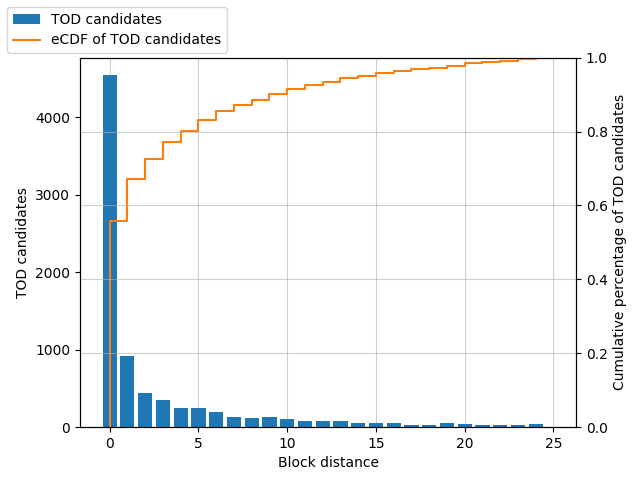
\includegraphics[width=0.8\textwidth]{charts/tod_candidates_block_dist.png}
    \caption[Block distances of TOD candidates]{The histogram and eCDF of the block distance for TOD candidates. The blue bars show how many TOD candidates have been found, where $T_A$ and $T_B$ are n blocks apart. The orange line shows the percentage of TOD candidates, that are at most n blocks apart.}
    \label{fig:tod_block_dist}
\end{figure}

\subsection{Collisions}

After applying our filters, we have 8818 storage collisions and 5654 balance collisions remaining. When we analyze, how often each account is part of a collision, we see that collisions are highly concentrated around a small set of accounts. For instance, the five accounts with the most collisions\footnote{All of them are token accounts: \href{https://etherscan.io/address/0xc02aaa39b223fe8d0a0e5c4f27ead9083c756cc2}{WETH}, \href{https://etherscan.io/address/0x97a9a15168c22b3c137e6381037e1499c8ad0978}{DOP}, \href{https://etherscan.io/address/0xdac17f958d2ee523a2206206994597c13d831ec7}{USDT}, \href{https://etherscan.io/address/0xa0b86991c6218b36c1d19d4a2e9eb0ce3606eb48}{USDC} and \href{https://etherscan.io/address/0xf938346d7117534222b48d09325a6b8162b3a9e7}{CHOPPY}} are responsible for 43.0\% of all collisions. In total, the collisions occur in only 1472 different account states.

One goal of this paper is to create a diverse set of attacks for our benchmark. With such a strong imbalance towards a few contracts, it will take a long time to analyze TOD candidates related to these frequent addresses, and the attacks are more likely related and do not cover a wide range of attack types. To prevent this, we may filter out duplicate addresses for collisions.

Figure \ref{fig:collsions_address_limit} depicts, how many collisions we would get when we only consider the first $n$ collisions for each address. If we set the limit to one collision per address, we would end up with 1472 collisions, which is exactly the number of unique addresses where collisions happened. When we keep 10 collisions per address, we would get 3964 collisions. Such a scenario would already reduce the amount of collisions by 73\%, while still retaining a sample of 10 collisions for each address, that could cover different types of TOD attacks.

\begin{figure}[h]
    \centering
    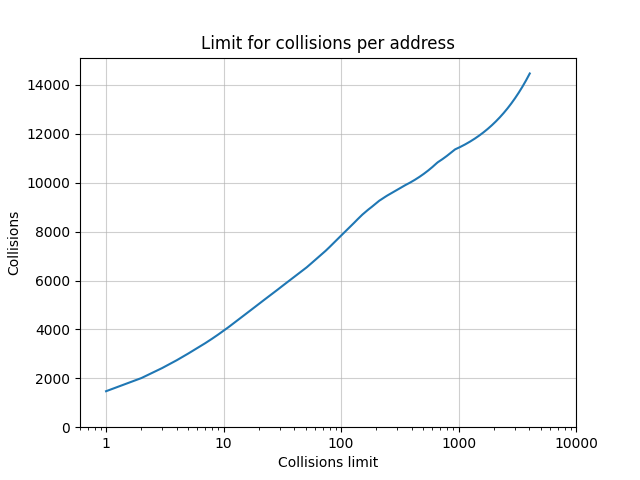
\includegraphics[width=0.8\textwidth]{charts/collisions_limited_per_address.png}
    \caption[Limit for collisions per address]{The chart shows, how many collisions we have, when we limit the number of collisions we include per address. For instance, if we only include 10 collisions for each address we would end up with about 4000 collisions.}
    \label{fig:collsions_address_limit}
\end{figure}

\section{Deduplication}

\todo{Consider implementing deduplication, e.g. filtering out collisions at the same address.}

\iffalse
    We want a diverse set of attacks for the benchmark, so we filter out similar attacks to the ones we already analyzed. For instance, it does not make sense to analyze 5000 attacks for the USDT Stablecoin, as these will mostly collide.

    If possible, we don't need the traces analyzer for deduplication. For instance, maybe we can get all the necessary information from the default RPC tracers.
    Alternatively, we could also download all necessary data, and then loop through the traces analyzer and only pick the relevant (deduplicated) potential attacks.

    Ideas, potentially a mixture of those:

    \begin{enumerate}
        \item only trace some attacks per contract
        \item only trace some attacks per function
        \item only trace some attacks per group of vulnerable contracts (as defined by analysis)
        \item only trace some attacks per contract/function skeletons
        \item similar to \cite{}, analyze at how many attacks per contract/function the number of found attacks saturate (based on the analysis result)
    \end{enumerate}
\fi

\chapter{Trace analysis}
\iffalse
    % For instance, all EVM transactions in the same block read and write to the beneficiary account for gas payment, making all transactions interdependent by default.
    % Is this the case? Do we see this in the prestate tracer?
    % https://github.com/risechain/pevm

    \section{Trace replaying}

    \subsection{Algorithm}

    Let's say, we have a transaction $T_A$ and a $T_B$, where $T_A$ occurred in block $Block_A$ and $T_B$ occurred in $Block_B$ (which may be equal to $Block_A$). Further, $T_A$ occurred before $T_B$, denoted as $T_A \rightarrow T_B$.

    We want to replay following scenarios:

    \begin{enumerate}
        \item actual: $T_A \rightarrow T_B$
        \item reverse: $T_B \rightarrow T_A$
    \end{enumerate}

    \subsubsection{Actual: $T_A \rightarrow T_B$}

    For $T_A$: We start with $\sigma_{B_A}$, being the world state at the start of the block containing $T_A$. Then we set $\sigma = \sigma_{B_A} + \sum_{i=0}^{i=index(T_A)}\Delta_{T(B_B)_i}$ and execute $\sigma \xrightarrow{T_A} \sigma\prime$.

    For $T_B$: We start with $\sigma_{B_B}$, being the world state at the start of the block containing $T_B$. Then we set $\sigma = \sigma_{B_B} + \sum_{i=0}^{i=index(T_B)}\Delta_{T(B_B)_i}$ and execute $\sigma \xrightarrow{T_B} \sigma\prime$.

    \subsubsection{Reverse: $T_B \rightarrow T_A$}


    For $T_B$: We start with $\sigma_{B_B}$, being the world state at the start of the block containing $T_B$. Then we set $\sigma = \sigma_{B_B} + (\sum_{i=0}^{i=index(T_B)}\Delta_{T(B_B)_i}) - \Delta_{T_A}$ and execute $\sigma \xrightarrow{T_B} \sigma\prime$.

    For $T_A$: We start with $\sigma_{B_A}$, being the world state at the start of the block containing $T_A$. Then we set $\sigma = \sigma_{B_A} + (\sum_{i=0}^{i=index(T_A)}\Delta_{T(B_B)_i}) + \Delta_{T_B\prime}$ and execute $\sigma \xrightarrow{T_A} \sigma\prime$.

    \section{Trace parsing}

    Features:

    \begin{enumerate}
        \item parses executed instructions with inputs and outputs
        \item handles internal transactions, including normal and exceptional halts
        \item tracks data origin for each byte of data, across calls and storages
        \item uses reference for DUPn instructions (so verification on one duplicate also verifies the other duplicate)
        \item outputs data flow graph, eg for source-sanitizers-sink analysis (and sanitizers could occur after sinks in Ethereum, because of reverts)
    \end{enumerate}

    Using traces instead of a full-fledged EVM allows:

    \begin{enumerate}
        \item easier extension, as for instructions we only need to model their data flow
        \item interoperability with all nodes and other tools that produce traces
        \item automatic verification of the modelled data flows against the actual stack and memory
    \end{enumerate}

    \subsection{Data flow graph}

    Horus and EVMTracer use a similar approach, by building a shadow state that contains the dependency information for each value.

    We use a different approach, where our shadow state is directly used for computation. Furthermore, our approach is on byte level. Furthermore, our approach tracks data dependencies, rather than instruction step dependencies (and idk yet what exactly the dis-/advantages of that are).

    \section{Attack categorization}

    \section{Vulnerability localization}

    \section{Attack labeling}
\fi
\chapter{TOD Attack results}

Overall findings of the TOD attack mining and analysis.

\chapter{Tool benchmarking}

\section{Systematic Literature Review}

\section{Result}

\chapter{Data availability}

TBD.

\chapter{Reproducibility}
\label{cha:reproducibility}

\section{Tool}

TBD.

\section{Randomness}

TBD.

\section{Experiment setup}

The experiments were performed on Ubuntu 22.04.04, using an AMD Ryzen 5 5500U CPU with 6 cores and 2 threads per core and a SN530 NVMe SSD. We used a 16 GB RAM with an additional 16 GB swap file.

For the RPC requests we used a public endpoint\cite{noauthor_pokt_2024}, which uses Erigon\cite{noauthor_rpc_2024} according to the \verb|web3_clientVersion| RPC method. We used a local cache to prevent repeating slow RPC requests. \cite{fuzzland_eth_2024} Unless otherwise noted, the cache was initially empty for experiments that measure the running time.

\backmatter

\begin{aitools}
    No generative AI tools where used in the process of researching and writing this thesis.
\end{aitools}

% Use an optional list of figures.
\listoffigures % Starred version, i.e., \listoffigures*, removes the toc entry.

% Use an optional list of tables.
\cleardoublepage % Start list of tables on the next empty right hand page.
\listoftables % Starred version, i.e., \listoftables*, removes the toc entry.

% Use an optional list of alogrithms.
\listofalgorithms
\addcontentsline{toc}{chapter}{List of Algorithms}

% Add an index.
\printindex

% Add a glossary.
\printglossaries

% Add a bibliography.
\bibliographystyle{alpha}
\bibliography{references}

\end{document}